\documentclass[a4paper,11pt]{article}
\usepackage[margin=1in]{geometry}
\usepackage{tikz,tkz-graph,graphicx}
\usepackage{xcolor}
\usepackage{subcaption}

\usetikzlibrary{arrows.meta,positioning,shapes,chains,calc,math}

\definecolor{lightOrange}{rgb}{0.9921875,0.890625,0.69921875}
\definecolor{darkOrange}{rgb}{0.96875,0.64453125,0.33203125}
\definecolor{skyBlue}{rgb}{0.66796875,0.875,0.97265625}
\definecolor{darkBlue}{rgb}{0.046875,0.69140625,0.9375}

\begin{document}

\section*{Picture}
\begin{figure}[h]
	\centering
	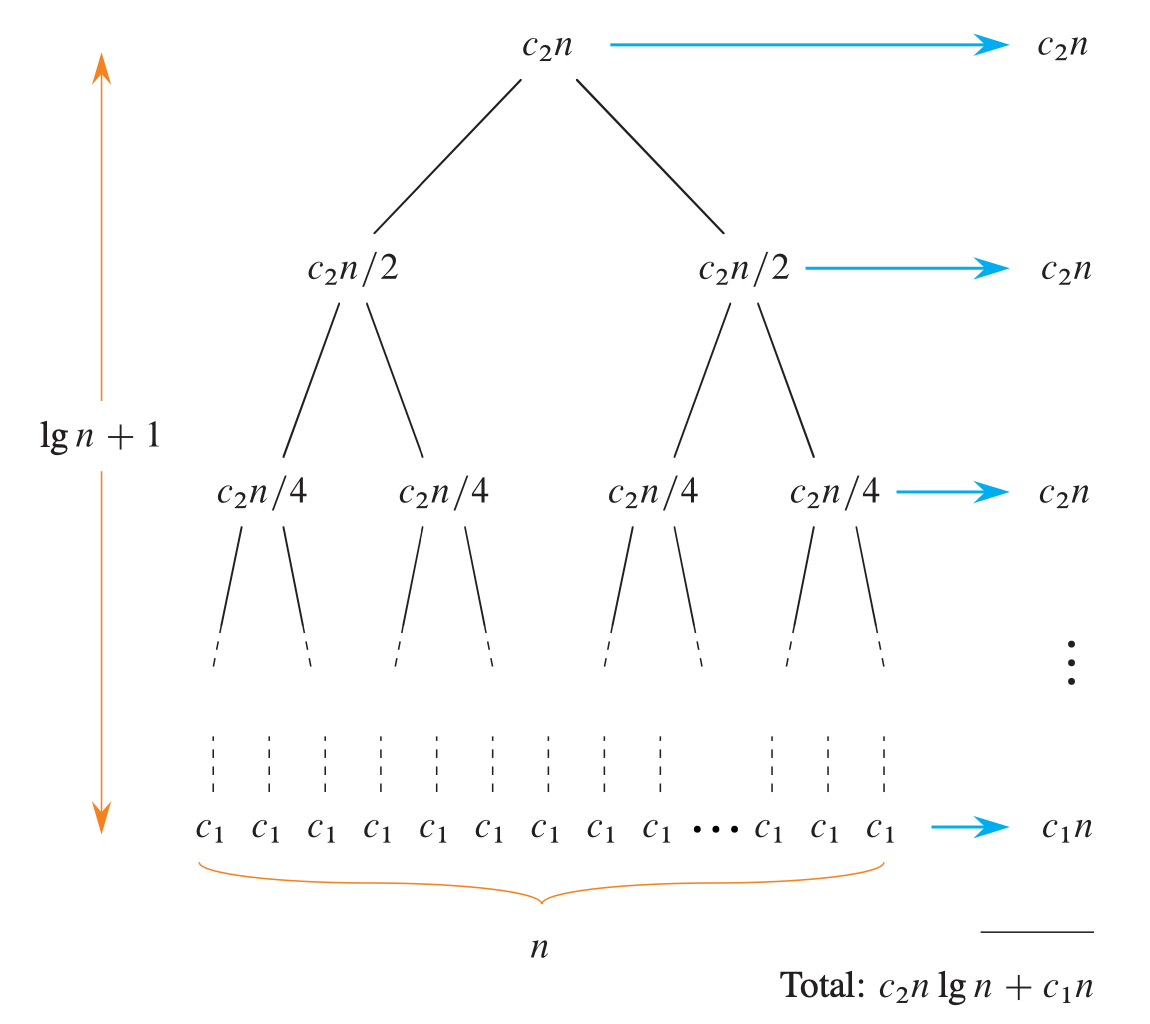
\includegraphics[width=0.67\textwidth]{./6.png}
\end{figure}

\section*{PDF}
\begin{figure}[ht]
\centering
  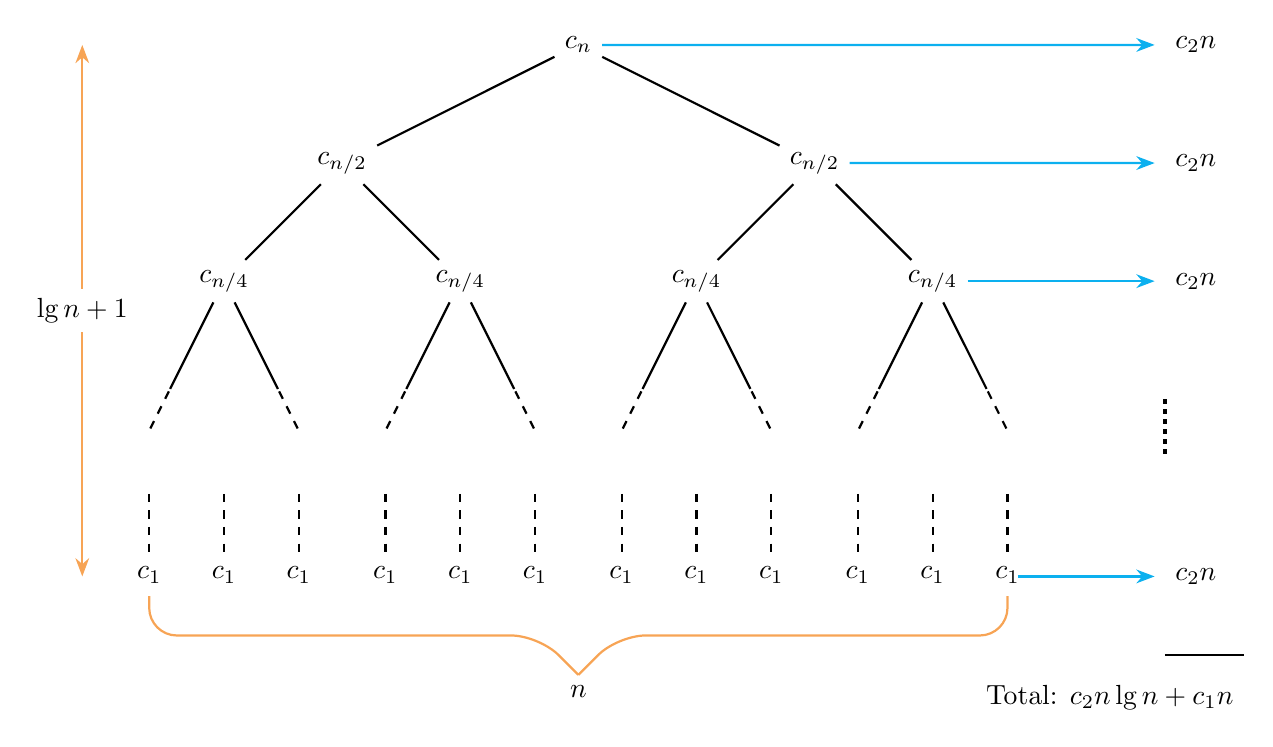
\begin{tikzpicture}[thick, >=Stealth]
    \node (right1) {$c_n$}
    child{ node{$c_{n/2}$}
      child{node (last1) {$c_{n/4}$}
        child{node (leaf1) {~}}
        child{node (leaf2) {~}}
      }
      child[missing]
      child{node (last2) {$c_{n/4}$}
        child{node (leaf3) {~}}
        child{node (leaf4) {~}}
      }
    }
    child[missing]
    child[missing]
    child[missing]
    child{ node (right2) {$c_{n/2}$}
      child{node (last3) {$c_{n/4}$}
        child{node (leaf5) {~}}
        child{node (leaf6) {~}}
      }
      child[missing]
      child{node (right3) {$c_{n/4}$}
        child{node (leaf7) {~}}
        child{node (leaf8) {~}}
      }
    }
    ;

    \foreach \i in {1,3,...,8}{
      \draw[dashed] ($(leaf\i)+(0.05,0.1)$) --
      ($(leaf\i)+(-0.2,-0.4)$);
    }

    \foreach \i in {2,4,...,8}{
      \draw[dashed] ($(leaf\i)+(-0.05,0.1)$) --
      ($(leaf\i)+(0.2,-0.4)$);
    }

    \foreach \i in {1,3,...,8}{
      \draw[dashed] 
      ($(leaf\i)+(-0.2,-1.2)$) --
      ($(leaf\i)+(-0.2,-2)$)
      node [below] {$c_1$}
      ;
    }

    \foreach \i in {2,4,...,8}{
      \draw[dashed] 
      ($(leaf\i)+(0.2,-1.2)$) --
      ($(leaf\i)+(0.2,-2)$)
      node [below] {$c_1$}
      ;
    }

    \draw[dashed]
    ($(right3)+(0,-2.7)$) -- ($(right3)+(0,-3.5)$)
    node [below] {$c_1$}
    ;

    \foreach \i in {1,...,3}{
      \draw[dashed]
      ($(last\i)+(0,-2.7)$) -- ($(last\i)+(0,-3.5)$)
      node [below] {$c_1$};
    }

    \node (right4) at ($(leaf8)+(0.2,-2.25)$) {};

    \node (level4) at ($(right4)+(2,0)$)      {};
    \node (level3) at ($(level4)+(0,3.75)$)    {};
    \node (level2) at ($(level3)+(0,1.5)$)   {};
    \node (level1) at ($(level2)+(0,1.5)$)   {};

    \foreach \i in {1,...,4}{
      \draw[->,thick,darkBlue]
      (right\i) -- (level\i)
      node[right,text=black] {$c_2n$}
      ;
    }

    \draw[dotted, ultra thick]
    ($(level3)+(0,-1.5)$) --
    ($(level4)+(0,1.5)$);

    \draw
    ($(level4)+(0,-1)$) --
    ($(level4)+(1,-1)$);

    \node at ($(level4)+(1,-1.25)$) [below left] {Total: $c_2n\lg
      n+c_1n$};

    \draw[rounded corners=10pt, thick, darkOrange]
    ($(leaf1)!0.5!(leaf8) + (0,-3.5)$)
    -- ++ (-0.5,0.5)
    --
    ($(leaf1)+(-0.2,-3)$)
    --
    ($(leaf1)+(-0.2,-2.5)$)
    ;
    \draw[rounded corners=10pt, thick, darkOrange]
    ($(leaf1)!0.5!(leaf8) + (0,-3.5)$)
    -- ++ (0.5,0.5)
    --
    ($(leaf8)+(0.2,-3)$)
    --
    ($(leaf8)+(0.2,-2.5)$)
    ;
    \node at ($(leaf1)!0.5!(leaf8) + (0,-3.5)$) [below] {$n$};

    \draw[<->, darkOrange]
    ($(level1)+(-13.75,0)$)
    --
    node[midway,fill=white,text=black] {$\lg n+1$}
    ($(level4)+(-13.75,0)$)
    ;
 \end{tikzpicture}
\end{figure}
\end{document}